\documentclass[t]{beamer}
\usepackage{hyperref}

\definecolor{rrblitbackground}{rgb}{0.55, 0.3, 0.1}

\newenvironment{rtbliteral}{

\begin{ttfamily}

\color{rrblitbackground}

}{

\end{ttfamily}

}

\usetheme{Warsaw}

\setbeameroption{hide notes}

% generated by Docutils <http://docutils.sourceforge.net/>
\usepackage{cmap} % fix search and cut-and-paste in Acrobat
\usepackage{ifthen}
\usepackage[T1]{fontenc}
\usepackage[latin1]{inputenc}
\usepackage{graphicx}
\usepackage{alltt}

%%% Custom LaTeX preamble
% PDF Standard Fonts
\usepackage{mathptmx} % Times
\usepackage[scaled=.90]{helvet}
\usepackage{courier}

%%% User specified packages and stylesheets

%%% Fallback definitions for Docutils-specific commands

% class handling for environments (block-level elements)
% \begin{DUclass}{spam} tries \DUCLASSspam and
% \end{DUclass}{spam} tries \endDUCLASSspam
\ifx\DUclass\undefined % poor man's "provideenvironment"
 \newenvironment{DUclass}[1]%
  {\def\DocutilsClassFunctionName{DUCLASS#1}% arg cannot be used in end-part of environment.
     \csname \DocutilsClassFunctionName \endcsname}%
  {\csname end\DocutilsClassFunctionName \endcsname}%
\fi

% hyperlinks:
\ifthenelse{\isundefined{\hypersetup}}{
  \usepackage[colorlinks=true,linkcolor=blue,urlcolor=blue]{hyperref}
  \usepackage{bookmark}
  \urlstyle{same} % normal text font (alternatives: tt, rm, sf)
}{}


%%% Body
\begin{document}

\begin{frame}[fragile]
\frametitle{Sage Combinat Widgets}


A collection of \textbf{interactive widgets} for the \emph{Jupyter} notebook
\begin{itemize}[<+-| alert@+>]

\item graphically represent

\item edit graphically and get the modified value

\item can be used as building blocks in applications

\item available for
\begin{itemize}[<+-| alert@+>]

\item (until now only grid-representable) combinatorial objects

\item (until now only grid-representable) graphs

\item matrices

\item write your own
\end{itemize}
\end{itemize}
\end{frame}

\begin{frame}[fragile]
\frametitle{Editing a Young Tableau}


1 image de tableau + 1 vid�o (lien)
\end{frame}

\begin{frame}[fragile]
\frametitle{Tossing Dominos}


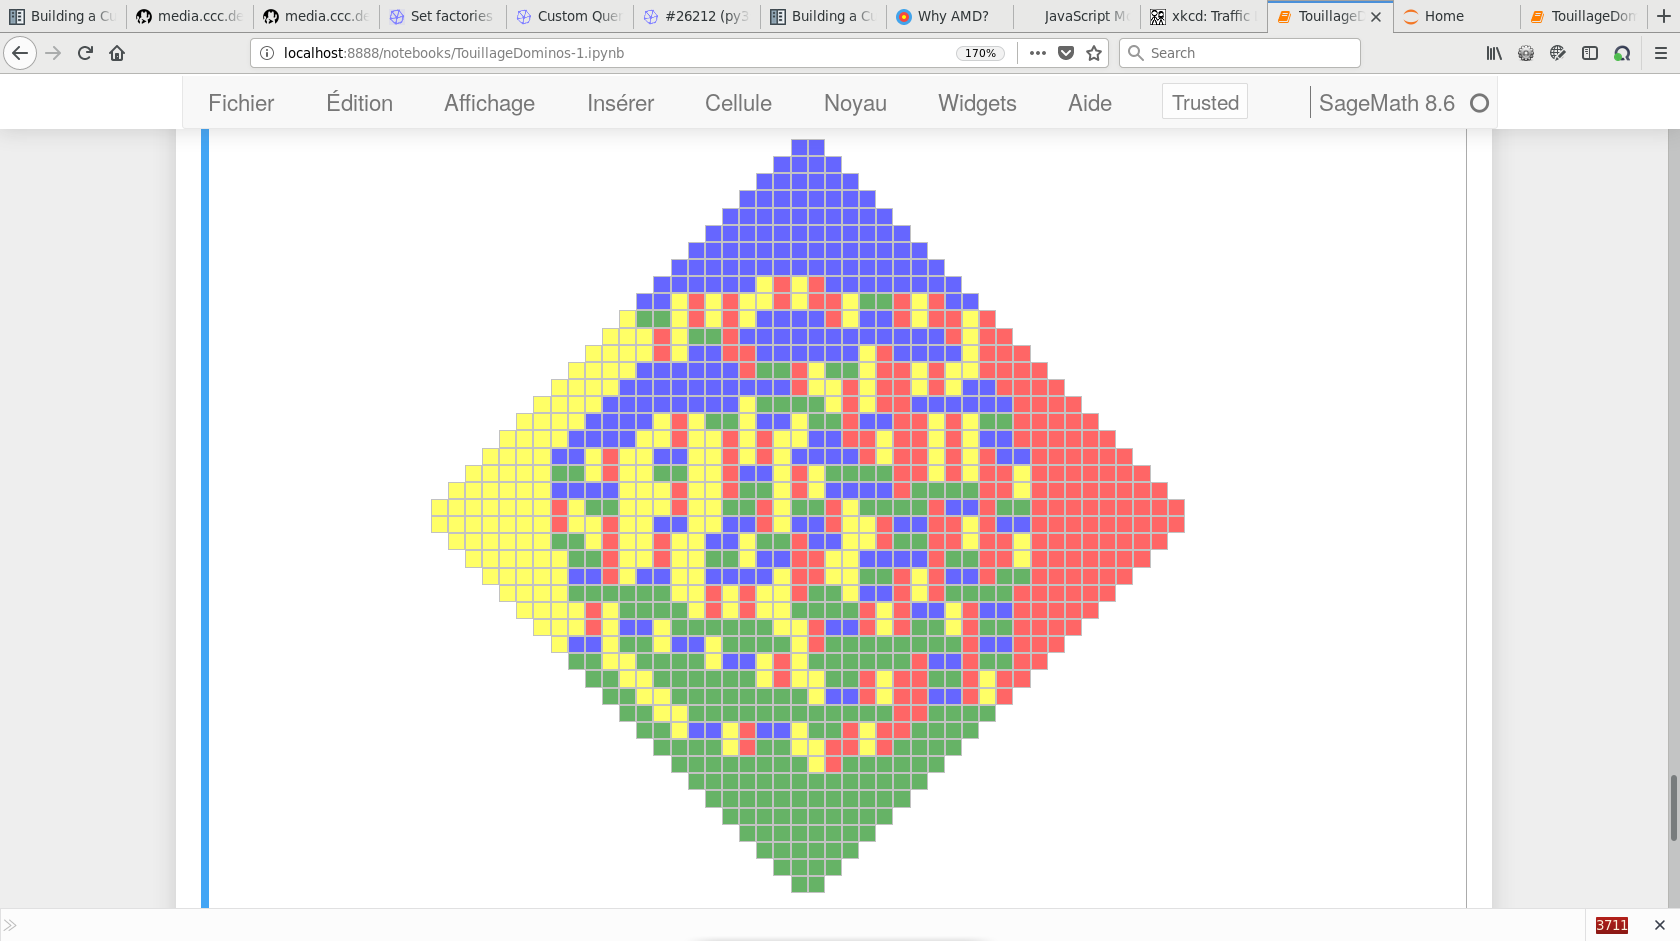
\includegraphics[scale=0.250000]{images/TossedDiamond22.png}

1 image de touillage + 1 vid�o (lien)

couplage ? (si j'y arrive : 1 image � mettre en-dessous ou � c�t�)
\end{frame}

\begin{frame}[fragile]
\frametitle{Using @interact}


1 image de products of Schur functions + vid�o (lien)
\end{frame}

\begin{frame}[fragile]
\frametitle{Your own widget: Jeu de Taquin example (1)}


1 image de jeu de taquin + vid�o
\end{frame}

\begin{frame}[fragile]
\frametitle{Your own widget: Jeu de Taquin example (2)}

\setbeamerfont{quote}{parent={}}

\begin{DUclass}{code-block}
\begin{quote}
\begin{alltt}
def myfunc (arg1, arg2='foo'):
        global baz
        bar = unicode (quux)
        return 25
\end{alltt}
\end{quote}
\end{DUclass}
\setbeamerfont{quote}{parent=quotation}
\end{frame}

\end{document}
